\documentclass[11pt]{article}
\usepackage[a4paper,margin= 2cm]{geometry}
\usepackage{graphicx}
\usepackage{caption}
\usepackage{subcaption}

\title{\LARGE{\bf{Task 4 - Quadrature}}}
\author{\Large{\bf{Kirtan Patel - AE19B038}}}
\date{}

\begin{document}

\maketitle 

\section{Introduction}
In mathematics, quadrature is a historical term which means the process of determining area. This term is still used nowadays in the context of differential equations, where "solving an equation by quadrature" or "reduction to quadrature" means expressing its solution in terms of integrals.\\

There are various reasons as of why such approximations
can be useful. First, not every function can be analytically integrated. Second, even if a
closed integration formula exists, it might still not be the most efficient way of calculating
the integral. In addition, it can happen that we need to integrate an unknown function,
in which only some samples of the function are known.\\

This report includes working and analysis of 4 methods of quadrature:
\begin{enumerate}
	\item Rectangular Method
	\begin{enumerate}
		\item Left Endpoint Rule
		\item Right Endpoint Rule
		\item Midpoint Rule
	\end{enumerate}
	\item Trapezoid Method
\end{enumerate}

\subsection{Rectangular Method}
In order to gain some insight on numerical integration, we review Riemann integration, a framework that can be viewed as an approach for approximating integrals.\\

We assume that \textit{f(x)} is bounded function defined on [a,b] and that {$x_0, . . . . ,x_n$} is a partition(P) of [a,b]. For each \textit{i} we let
\[ M_i(f) = \mathop{sup}_{x\in[x_{i-1},x_i]} f(x)\] and \[m_i(f) = \mathop{inf}_{x\in[x_{i-1},x_i]} f(x)\]
Thus, $M_i(f)$ represents the Maxima of f(x) in the ith interval [$x_{i-1},x_{i}]$ while $m_i(f)$ represents the Minima of f(x) in the ith interval [$x_{i-1},x_{i}]$.\\
Letting $\delta x_i = x_i - x_{i-1}$ , the \textbf{upper (Darboux) sum} of f(x) with respect to the partition P is defined as : 
\[ U(f,P) = \sum_{i=1}^{n}M_i\Delta x_i\] 
while the \textbf{lower (Darboux) sum} of f(x) with respect to the partition P is defined as : 
\[ L(f,P) = \sum_{i=1}^{n}m_i\Delta x_i\] \\

The upper bound integral of f(x) on [a,b] is defined as :
\[ U(f)= inf(U(f,P))\]
and the lower bound integral of f(x) is defined as
\[ L(f)= sup(L(f,P))\] where both the infimum and the supremum are taken over all possible partitions, P, of the interval [a,b]. \\

As mentioned above, the bound estimation of integral $\int_{a}^{b}f(x) \,dx$ can be done using the extremum values attained by the function in the given range. However, these sums are not defined in the most convenient way for an approximation algorithm. This is because we need to find the extrema of the function in every subinterval. Finding the extrema of the function, may be a complicated task on its own, which we would like to avoid.\\

A simpler approach for the approximation is to compute the product of the value of the function ar either of the end-points of the interval by the length of the interval. For an increasing function, taking the left endpoint would give a lower bound value while the right endpoint would give an upper bound value. The opposite is true if the function is decreasing.\\

A variation on the rectangular rule is the midpoint rule. Similar to the rectangular rule, we approximate the value of the integral by multiplying the length of the interval by the value of the function at one point. Only this time, we use the value of the function at the center point of the interval.\\

\begin{figure} [h!]
	\centering
	\begin{subfigure}{0.5\textwidth}
		\centering
		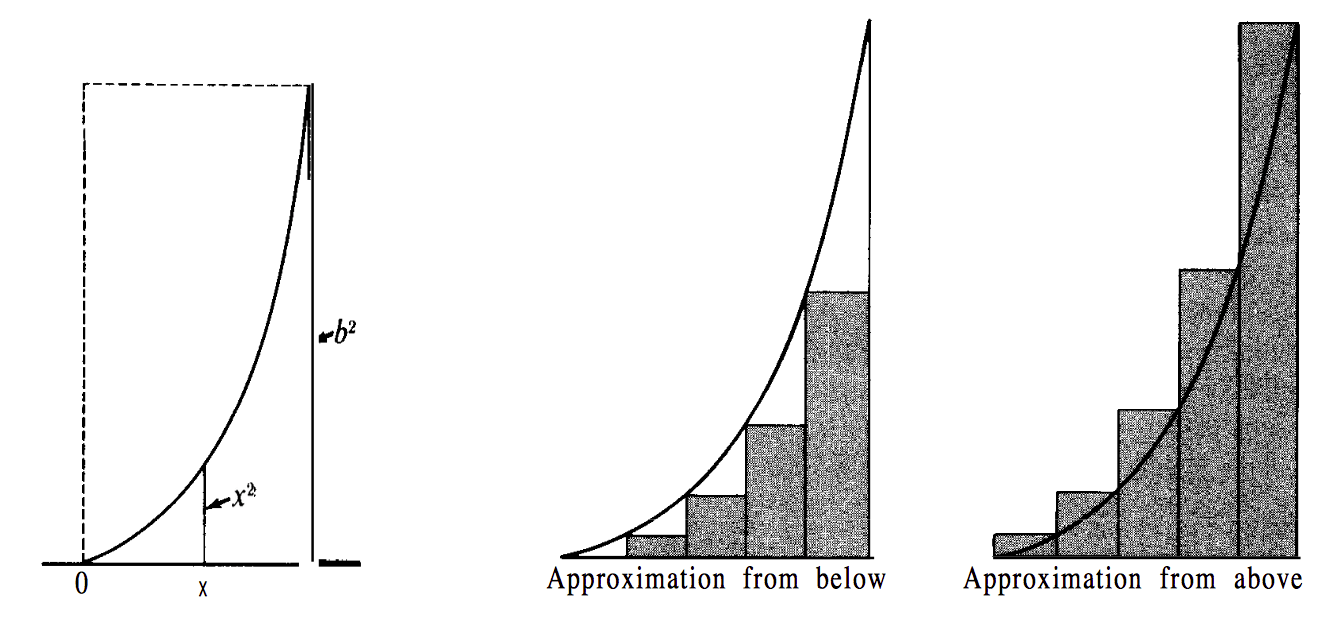
\includegraphics[width=1.1\linewidth]{Sample1}
		\label{fig1:sub1}
	\end{subfigure}%
	\hspace{1cm}
	\begin{subfigure}{0.4\textwidth}
		\centering
		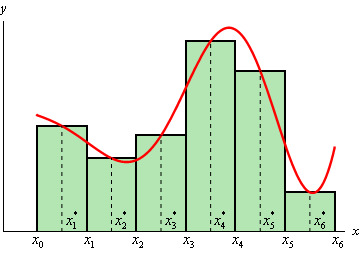
\includegraphics[width=0.9\linewidth]{Sample2}
		\label{fig1:sub2}
	\end{subfigure}
	\caption{Graphical Representation of Quadrature using Rectangular Rule}
\end{figure}

\subsection{Trapezoid Method}
This technique is a much more accurate way to 
approximate area beneath a curve.  To construct the 
trapezoids, you mark the height of the function at the beginning and end of the width interval, then connect the two points.
We get a better approximation of graphs which are closer to linear, by assuming each interval to be consisting of trapeziums. Here we use both the end-points and average the values at the endpoints.\\

On dividing the integration interval into sub-intervals, this is termed as the composite trapezoid rule, which is obtained by applying the trapezoid rule in each sub-interval and then adding the resulting areas together\\

The Trapezoidal Rule overestimates a curve that is 
concave up and underestimates functions that are 
concave down.

\begin{figure} [h!]
	\centering
	\begin{subfigure}{0.5\textwidth}
		\centering
		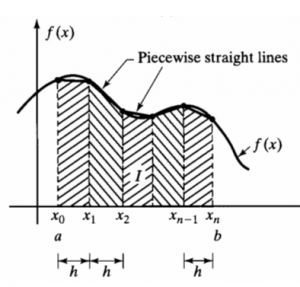
\includegraphics[width=0.8\linewidth]{Sample3}
		\label{fig2:sub2}
	\end{subfigure}%
	\begin{subfigure}{0.5\textwidth}
		\centering
		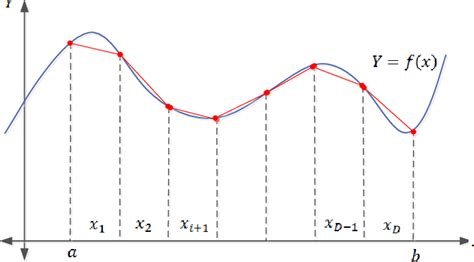
\includegraphics[width=0.8\linewidth]{Sample4}
		\label{fig2:sub3}
	\end{subfigure}
	\caption{Graphical Representation of Quadrature using Rectangular Rule}
\end{figure}
\vspace{1cm}
\subsection{Remarks}
There are several other method which use weighted averages of the areas and give a less errorneous result.The following are a few of them:
\begin{itemize}
	\item \textbf{Newton-Cotes Methods}
	Use intepolating polynomials. Trapezoid, Simpson’s 1/3 and 3/8 rules,
	Bode’s are special cases of 1st, 2nd, 3rd and 4th order polynomials are
	used, respectively
	\item \textbf{Romberg Integration(Richardson Extrapolation)}
	uses knowledge of error estimated to build a recursive higher order scheme
	\item \textbf{Gauss Quadrature}
	Like Newton-Cotes, but instead of a regular grid, choose a set that lets you get higher order accuracy
	\item \textbf{Monte Carlo Integration}
	Use randomly selected grid points. Useful for higher dimensional integrals (d>4)
\end{itemize}

\pagebreak

\section{Results and Analysis}
Taking the number of sub-intervals from the user, and finding the error in the quadrature found by each method, we get the following results.
\subsection{Absolute Error vs $\Delta$x}
\begin{figure}[h!]
	\centering
	\centering
	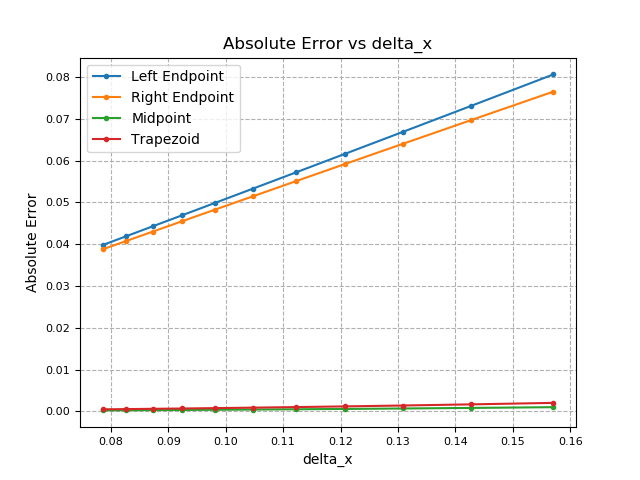
\includegraphics[width=0.8\linewidth]{abs_error}
	\caption{Absolute Error vs $\Delta x$ size of sub-interval}
	\label{fig4}
\end{figure}

\subsection{log(Absolute Error) vs $\Delta$x}
\begin{figure} [h!]
	\centering
	\begin{subfigure}{0.55\textwidth}
		\centering
		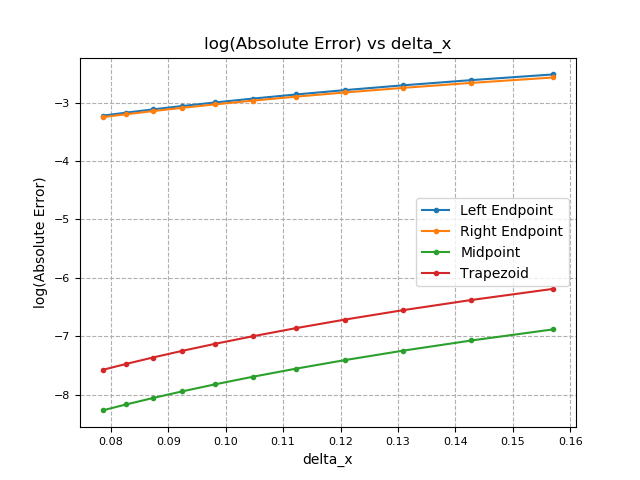
\includegraphics[width=\linewidth]{log_abs_error}
		\caption{log(absolute error) vs $\Delta$x}
		\label{fig2:sub1}
	\end{subfigure}%
	\begin{subfigure}{0.55\textwidth}
		\centering
		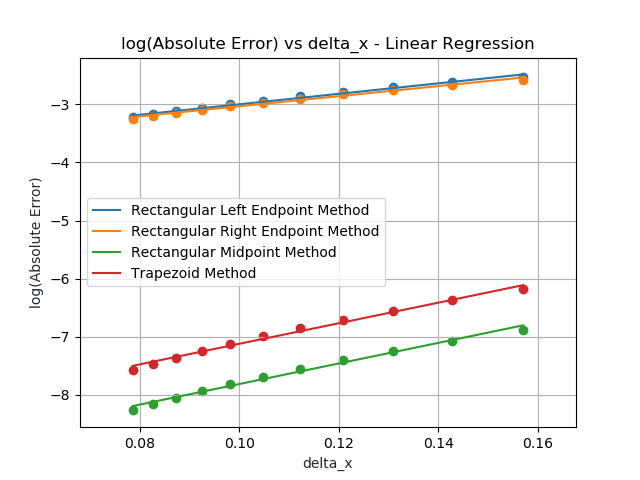
\includegraphics[width=\linewidth]{log_error_vs_delta_x_Lin_Reg}
		\caption{log(absolute error) vs $\Delta$x - Linear Regression}
		\label{fig2:sub2}
	\end{subfigure}
	\caption{Results obtained by plotting log(Absolute Error) vs $\Delta$x}
\end{figure}
We can see that the Midpoint and Trapezoid Rules give a far more accurate result than the Left and Right Endpoint Rules. This difference is significant in functions with large slopes and large slope changes.\\

Furthermore, the Midpoint Rule gives a slightly better result than the Trapezoid Rule. For more linear functions, this difference negligible while for highly non-linear functions, the difference is large.\\

We can even see that the relation is almost linear between the Absolute error and the size of the sub-interval. Naturally, if we use a finer sub-interval, we go closer and closer to the true value of the integral and hence the error tends to zero.\\

It is important to note that the user inputs the number of intervals the integration interval is to be divided in. The sub-interval size $\Delta$x is given by : \[ \Delta x = \frac{(upper~integration~limit - lower~integration~limit)}{number~of~sub-intervals}\]
\subsection{Absolute Error vs Number of Sub-intervals}

\begin{figure}[h!]
	\centering
	\centering
	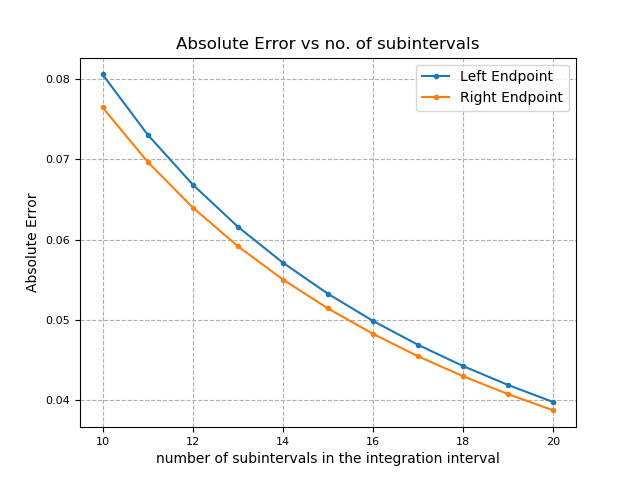
\includegraphics[width=0.8\linewidth]{abs_error_vs_num_subintervals}
	\caption{Result obtained by plotting Absolute Error vs number of sub-intervals}
	\label{fig4}
\end{figure}

We can see that the Absolute Error is \textbf{inversely proportional} to the number of sub-intervals. \\

This is even verified by seeing the Absolute Error vs $\Delta$x plot which is linear. This, along with the relation between $\Delta$x and number of sub-intervals confirms that the plot lines with the mathematical relation y $\propto$ $\frac{1}{x}$ \\

As the number of subintervals tends to $\infty$, the Absolute Error tends to 0
\pagebreak

\section{Order of Accuracy}
The 'order of accuracy' is a way to quantify the accuracy of the method i.e. how close the output of the method si to the actual value. Since the value we get from numerical method is an approximation to the actual value, there is an error value which is greater than zero, as the approximate value is not exactly the same as the actual value but close to it. The error value is found to depend on the 'step-size' that is used, and the error decreases if we decrease the step-size and we get more "accurate" result as the approximation value inches closer to the actual value.\\

We get the error dependence on the step-size as : 
\[ E(h) = Ch^n\]
where :
\begin{itemize}
	\item \textbf{E(h)} is the error which is dependent on the step-size
	\item \textbf{h} is the step-size
	\item \textbf{C} is a constant
\end{itemize}
Here the value \textbf{n} gives the order of accuracy.\\

The degree of accuracy of a Quadrature Formula is the largest positive integer n such that the formula is for x$^k$ for each k = 0,1,...n.\\

The integral is given as : 
\[ \int_{a}^{b}f(x) \,dx = Numerical~Integral~+~Error\]
In terms of the above defition, the order of accuracy is the highest degree of a polynomial for which the Integration Method gives no error.
\subsection{Rectangular Rule}
The Left Endpoint Rectangular Rule follows : 
\[\int_{a}^{b}f(x) \,dx = {b-a}[f(a)]~+~Error\]
The Right Endpoint Rectangular Rule follows : 
\[\int_{a}^{b}f(x) \,dx = {b-a}[f(b)]~+~Error\]
The Midpoint Rectangular Rule follows : 
\[\int_{a}^{b}f(x) \,dx = {b-a}[f(\frac{a+b}{2})]~+~Error\] \\

Let f(x) = x$^0$\\
For which integral value~~$\int_{a}^{b} x^0 \,dx~=~\int_{a}^{b} 1 \,dx~=~ b-a$\\
And the Rectangular Rule (for all the 3 sub-rules) gives value: $(b-a).[1]~=~b-a$ \\
Hence there is \textbf{No Error} for x$^0$ \\
\pagebreak

For f(x) = x$^1$\\
For which integral value~~$\int_{a}^{b} x \,dx~=~\frac{b^2-a^2}{2}$\\
the Left Endpoint Rectagular Rule gives value: $(b-a).[a]~=~ab-a^2$\\
the Right Endpoint Rectagular Rule gives value: $(b-a).[b]~=~b^2-ab$\\
the Midpoint Rectagular Rule gives value: $(b-a).[\frac{a+b}{2}]~=~\frac{b^2-a^2}{2}$\\
Hence there is \textbf{No Error} for x$^1$ in the Midpoint Rule, while there is \textbf{Error} for the Left Endpoint and the Right Endpoint Rules.\\

But for f(x) = x$^2$\\
For which integral value~~$\int_{a}^{b} x^2 \,dx~=~\frac{b^3-a^3}{3}$\\
And the Midpoint Rectangular Rule gives value~= $\frac{b-a}{2}~[(\frac{a~+~b}{2})^2]$\\
Here there is a \textbf{ Error} for f(x) = x$^2$.\\

Therefore, the order of accuracy for the Midpoint Rectangular method is 1,\\
while the order of accuracy for the Left and Right Endpoint Rules is 0.
\subsection{Trapezoid Rule}
The Trapezoid Rule follows that : 
\[ \int_{a}^{b}f(x) \,dx = \frac{b-a}{2}[f(a)+f(b)]~+~Error\]

Let f(x) = x$^0$\\
For which integral value~~$\int_{a}^{b} x^0 \,dx~=~\int_{a}^{b} 1 \,dx~=~ b-a$\\
And the Trapezoid Rule gives value~= ~ $\frac{b-a}{2}~[1~+~1]~=~b-a$\\
Hence there is \textbf{No Error} for x$^0$ \\

Similarly Let f(x) = x$^1$\\
For which integral value~~$\int_{a}^{b} x \,dx~=~\frac{b^2-a^2}{2}$\\
And the Trapezoid Rule gives value~= ~ $\frac{b-a}{2}~[a~+~b]~=~\frac{b^2-a^2}{2}$\\
Hence there is \textbf{No Error} for x$^1$ as well.\\

But for f(x) = x$^2$\\
For which integral value~~$\int_{a}^{b} x^2 \,dx~=~\frac{b^3-a^3}{3}$\\
And the Trapezoid Rule gives value~= ~ $\frac{b-a}{2}~[a^2~+~b^2]$\\
Here there is a cubic\textbf{ Error} for f(x) = x$^2$.\\

Therefore, the the order of accuracy for the Trapezoid method is 1.\\

As we begin to use interpolation and other mathematical techniques, we can get a higet order of accuracy. e.g. The Simpson's 1/3 rule has an order of accuracy of 3.\\

Tabulating the order of accuracy(OoA) calculated,\\
\begin{table} [h!]
	\centering
\begin{tabular}{| l || l |}
	\hline
	Quadrature Method & OoA  \\
	\hline \hline
	Left Endpoint Rectangular Method & 0\\
	\hline 
	Right Endpoint Rectangular Method & 0 \\
	\hline 
	Midpoint Rectangular Method & 1 \\
	\hline
	Trapezoid Method & 1 \\
	\hline
\end{tabular}
\end{table}

This is seen evidently in the Absolute Error vs $\Delta$x plots (Figure 3 and Figure 4)

\section{References}
\begin{enumerate}
	\item https://en.wikipedia.org/wiki/Quadrature$\_$(mathematics)
	\item https://math.stackexchange.com/questions/2873291/what-is-the-intuitive-meaning-of-order-of-accuracy-and-order-of-approximation
	\item http://www.math.pitt.edu/~sussmanm/2070Fall07/lab$\_$10/index.html
	\item https://www.kth.se/social/upload/5287cd2bf27654543869d6c8/Ant-OrderofAccuracy.pdf
	\item https://www3.nd.edu/~zxu2/acms40390F11/sec4-3-Numerical$\_$integration.pdf
\end{enumerate}




\end{document}